\section{Implementation}
\label{g1:sec:implementation}  % TODO Adopt group prefix

\subsection{Query by Gesture Architecture}
\begin{figure}[H]
    \centering
    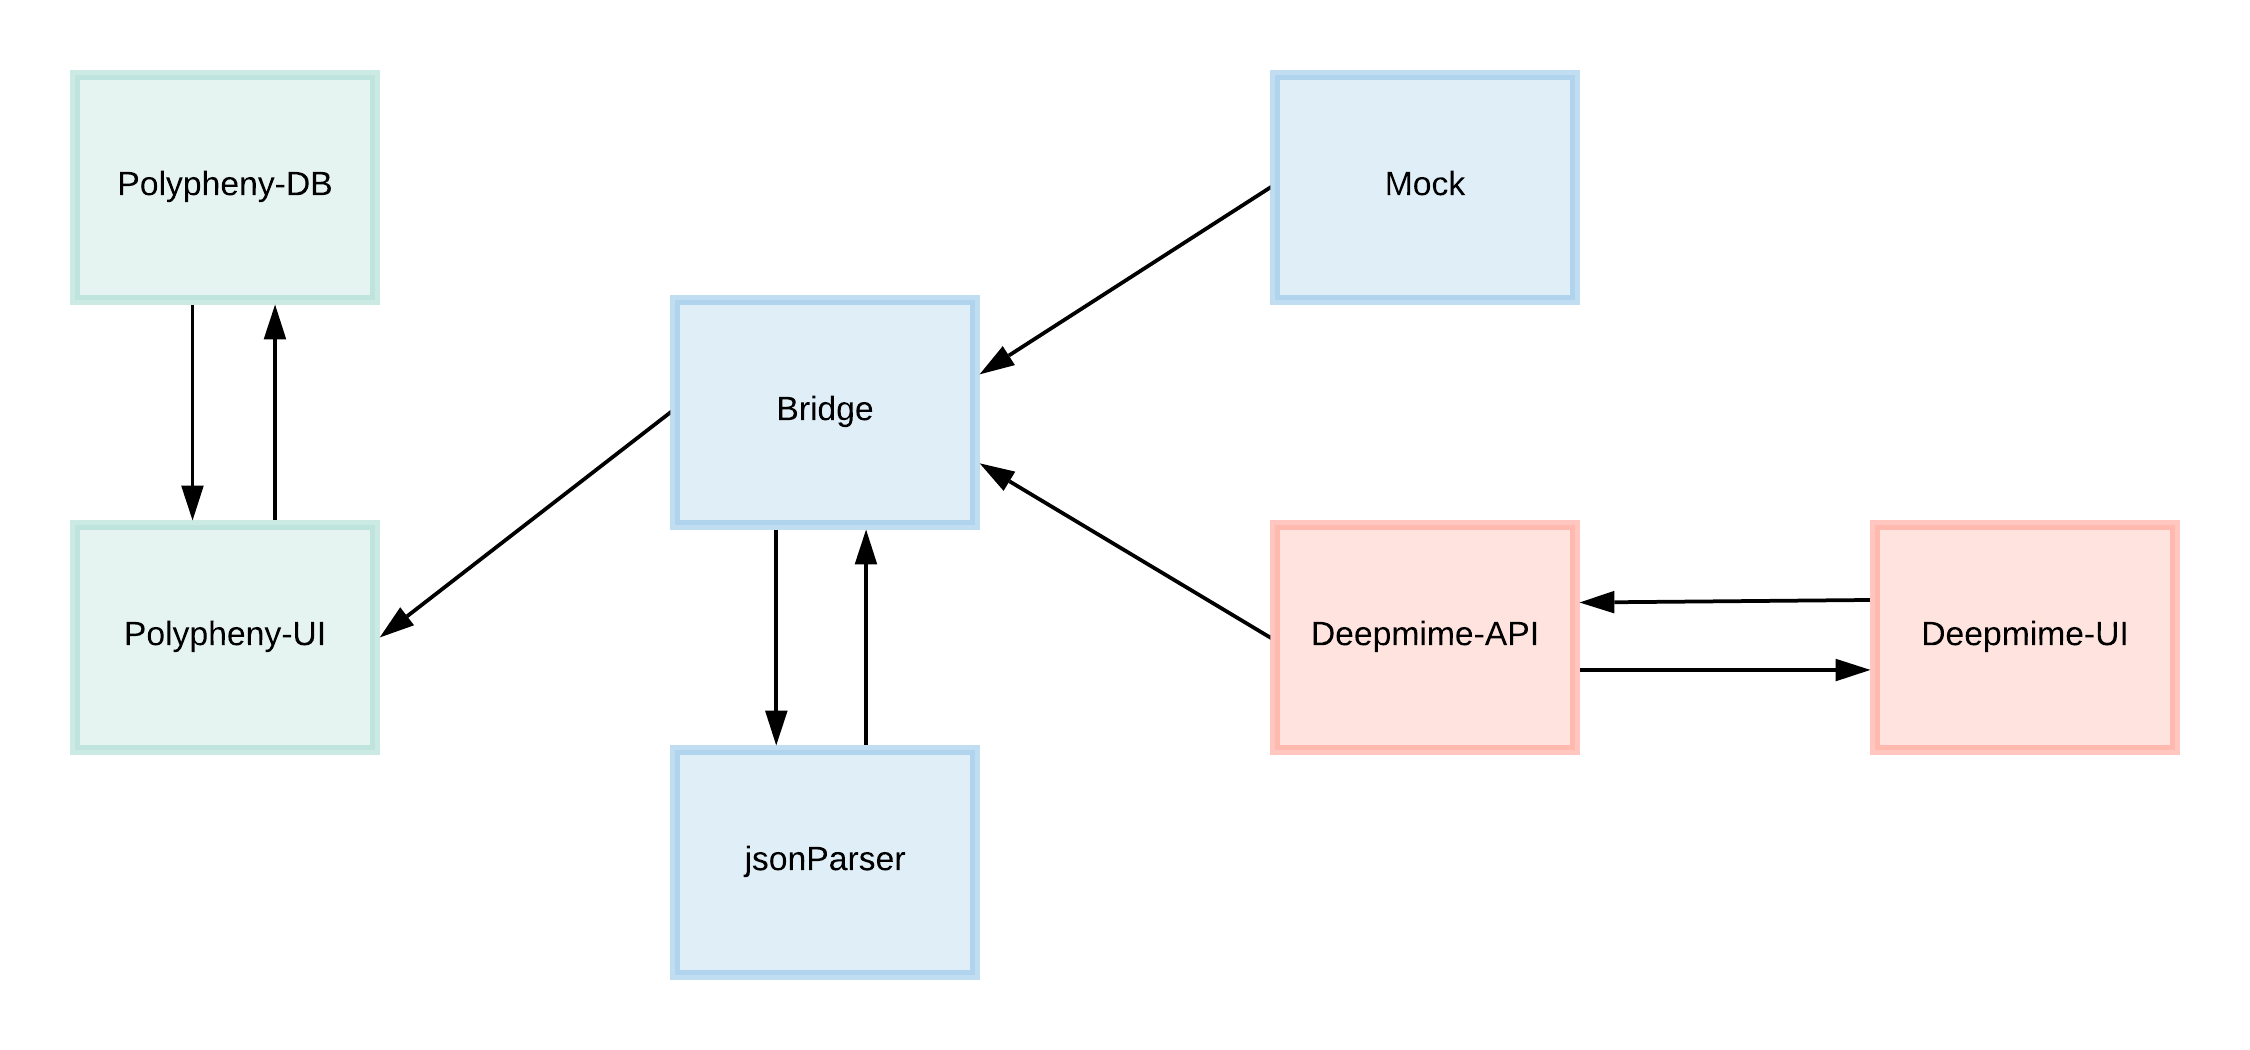
\includegraphics[width=\textwidth]{reportContent/images/QBG-Bridge.png}
    \caption{Overview Architecture Diagram}
    \label{fig:overall_architecture}
\end{figure}{}

\\
\\
As seen above in Figure \ref{fig:overall_architecture} the architecture of the project can be split into three modules: Polypheny (cyan), Query by Gesture Bridge (blue) and Deepmime (red).
Deepmime classifies gestures from a live video and sends them to the Query by Gesture Bridge. There they are processed and alter the relational query which is stored as a JSON object. This string then gets transferred to the Polypheny module where it gets displayed and in the end, the query can get executed. The modules are connected via a WebSockets. 

\subsection{Deepmime}
Deepmime is split into the UI and the API. In the UI you can upload a video or do life gesture recognition. The segments from the videos are sent to the API where they are classified. The classification is then again displayed in the UI.
In the API, after the video segment has been classified, the results get analysed. If the same gesture was detected several times in a row and its classification score is higher than a certain threshold it is sent to the server in the Query by Gesture Bridge. The UI is written in Angular and the API in Python.

\subsection{Query by Gesture Bridge}
As the name already suggests, this module serves as a bridge between the two other modules. The server acts as the WebSocket server between the two other modules. It takes gestures from Deepmime and translates them into a query plan in a JSON string that is then sent to Polypheny. The translation is done in the jsonParser. This class takes a gesture and executes the command the gesture is allocated to. Depending on that command it can add a new operator, change the specification of an operator or delete the last or all inserted operators. It also automatically calculates the position of all the operators that form the query. Additionally, this module also holds the mock file. It mocks the Deepmime module and is also able to connect to the server and send gestures. This whole module is written in Python.


\subsection{Polypheny}
This module only uses the polypheny-UI part of the whole Polypheny. An over-view of the used components and services can be seen in Figure \ref{fig:polypheny_architecture}. The \textit{right-sidebar.component} takes the connection details (ip:port) for the WebSocket connection and saves them in the \textit{webui-settings.service}. The "connect"/"disconnect" button starts/ends the WebSocket connection to the Query by Gesture Bridge. It does that by communicating with the \textit{relational-algebra.component} over the \textit{rightsidebar-to-relationalalgebra.service}. The \textit{relational-algebra.component} then activates the \textit{web-socket.service} which gets the connection details from \textit{webui-settings.service} and connects/disconnects to the Query by Gesture Bridge. Once the connection is established, the \textit{web-socket.service} listens and sends any incomming JSON objects to the \textit{relational-algebra.component} which then processes it, either by updating the query or deleting it. The Polypheny-UI is also written in Angular. As usual in Angular, the components are built from a typescript, a CSS and an HTML file. The services are only a typescript file.

\begin{figure}[H]
    \centering
    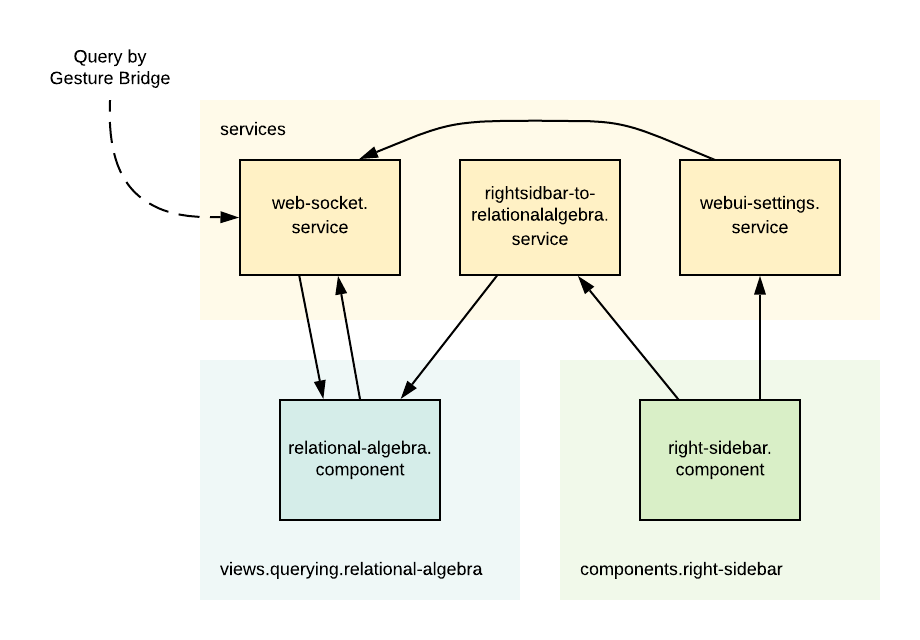
\includegraphics[width=\textwidth]{reportContent/images/PolyphenySchema.png}
    \caption{Components and Services used by Project in Polypheny-UI}
    \label{fig:polypheny_architecture}
\end{figure}{}